\documentclass[12pt,a4paper]{article}

\usepackage[a4paper,margin=1in]{geometry}
\usepackage{setspace}
\usepackage{titlesec}
\usepackage{graphicx}
\usepackage{longtable}
\usepackage{xcolor}
\usepackage{hyperref}
\usepackage{placeins}
\usepackage{enumitem}

% Compact section spacing
\titlespacing*{\section}{0pt}{12pt plus 4pt minus 2pt}{6pt plus 2pt minus 2pt}
\titlespacing*{\subsection}{0pt}{10pt plus 3pt minus 2pt}{4pt plus 2pt minus 2pt}

\onehalfspacing

\begin{document}

% ==================================================
% COVER PAGE
% ==================================================
\begin{titlepage}
\centering

\vspace*{2cm}

{\Huge \textbf{User Manual}}\\[0.5cm]
{\LARGE \textbf{CodeClash Arena}}\\[2cm]

\textbf{Group Number: XX}\\[0.5cm]
\textbf{Member Names and IDs}\\[3cm]

\textbf{Department of Computer Science and Engineering}\\
\textbf{University Name}\\[1cm]

\textbf{\today}

\vfill
\end{titlepage}

% ==================================================
% TABLE OF CONTENTS
% ==================================================
\tableofcontents
\newpage

% ==================================================
\section{Introduction}

\subsection{Purpose of the Manual}

This user manual serves as a comprehensive guide for users of CodeClash Arena, a gamified competitive programming platform designed to transform traditional coding practice into an interactive and engaging experience. The manual provides detailed instructions on how to use the platform effectively, from account creation to participating in competitive battles and clan wars.

This document is intended for:
\begin{itemize}
\item Beginner programmers seeking to improve their algorithmic skills through competitive practice
\item CSE students looking for engaging coding challenges
\item Competitive programming enthusiasts wanting real-time head-to-head battles
\item Coding instructors and educators implementing gamified learning environments
\item Clan leaders organizing team-based coding competitions
\end{itemize}

The manual covers all essential features of the platform, including step-by-step instructions, visual guidance through screenshots, troubleshooting tips, and best practices for optimal user experience. Whether you are a first-time user or an experienced programmer, this guide will help you navigate the platform efficiently and make the most of its features.

\subsection{Brief Overview of the Web Application}

CodeClash Arena is a web-based competitive programming platform that combines the excitement of multiplayer gaming with professional coding contests. Inspired by popular competitive games like Clash Royale and Clash of Clans, and integrated with the Codeforces problem repository, the platform offers a unique blend of entertainment and skill development.

\subsubsection{Core Concept}

Unlike traditional coding platforms that focus solely on individual practice, CodeClash Arena introduces real-time competitive elements including:
\begin{itemize}
\item \textbf{1v1 Coding Battles}: Challenge other coders in head-to-head real-time competitions
\item \textbf{Clan System}: Form or join teams and participate in clan-based battles
\item \textbf{Rating System}: Track your progress through an ELO-based ranking mechanism
\item \textbf{Practice Gym}: Solo practice mode with access to thousands of programming problems
\item \textbf{Matchmaking}: Automatic pairing with opponents of similar skill levels
\end{itemize}

\subsubsection{Key Differentiators}

CodeClash Arena addresses limitations of conventional coding platforms by providing:
\begin{itemize}
\item Direct head-to-head competition with other coders in real-time
\item Clan-based team competitions fostering collaboration and community
\item Personalized contest creation with custom difficulty and time settings
\item Gamified progression system with levels, XP, and visual achievements
\item Real-time battle synchronization showing opponent progress
\item AI-assisted learning through logical hints during practice sessions
\end{itemize}

\subsubsection{Technical Foundation}

The platform is built using modern web technologies:
\begin{itemize}
\item \textbf{Frontend}: React 19.2.0 with Vite 7.2.4 for fast, responsive user interface
\item \textbf{Backend}: Node.js with Express 4.18.2 for server-side logic
\item \textbf{Database}: Supabase (PostgreSQL) for data management
\item \textbf{Problem Integration}: Codeforces API for accessing thousands of programming problems
\item \textbf{Code Execution}: Piston API for local testing and Codeforces judge for official verdicts
\end{itemize}

\subsubsection{Platform Features Summary}

\begin{longtable}{|p{3.5cm}|p{10cm}|}
\hline
\textbf{Feature} & \textbf{Description} \\
\hline
\endhead

Global Battle Mode & Join a matchmaking queue and compete against players of similar rating in real-time 1v1 battles \\
\hline

Local Battle Mode & Challenge specific friends directly with customizable problem difficulty and time limits \\
\hline

Clan Wars & Form teams, compete in clan-based tournaments, and track team performance \\
\hline

Practice Gym & Access solo practice mode with filtering by difficulty, tags, and rating range \\
\hline

Rating System & ELO-based skill rating that adapts based on opponent strength and battle outcomes \\
\hline

Progression System & Earn experience points and level up through battles and problem solving \\
\hline

Leaderboards & Global and clan rankings updated in real-time showing top performers \\
\hline

Battle History & Comprehensive records of past matches, opponents, and performance metrics \\
\hline

Code Editor & Integrated syntax-highlighted editor supporting C++, Java, Python, JavaScript, and more \\
\hline

AI Hints & Logical approach guidance during practice sessions without revealing solutions \\
\hline

Social Features & Friend lists, clan chat, mail system, and player profile viewing \\
\hline

\end{longtable}

\FloatBarrier

% ==================================================
\section{System Requirements}

This section outlines the technical prerequisites and environmental requirements necessary to access and use CodeClash Arena effectively. Ensuring your system meets these specifications will provide optimal performance and user experience.

\subsection{Supported Browsers and Devices}

\subsubsection{Web Browsers}

CodeClash Arena is a web-based application accessible through modern web browsers. For the best experience, we recommend using the latest stable versions of the following browsers:

\begin{longtable}{|p{3cm}|p{3cm}|p{7.5cm}|}
\hline
\textbf{Browser} & \textbf{Minimum Version} & \textbf{Recommended Features} \\
\hline
\endhead

Google Chrome & Version 84+ & Best performance with V8 JavaScript engine, full CSS Grid and Flexbox gap support, excellent developer tools \\
\hline

Mozilla Firefox & Version 103+ & Strong privacy features, backdrop-filter support, reliable WebSocket connections, modern CSS features \\
\hline

Microsoft Edge & Version 84+ & Chromium-based engine, native Windows integration, excellent performance, full modern CSS support \\
\hline

Safari & Version 15+ & Optimized for macOS/iOS devices, complete modern CSS/JS feature support including aspect-ratio and flex gap \\
\hline

Opera & Version 84+ & Chromium-based, built-in VPN support, efficient resource usage, modern web standards compliance \\
\hline

Brave & Version 1.42+ & Privacy-focused, Chromium-based, full ES2020+ support, modern CSS Grid and Flexbox features \\
\hline

\end{longtable}

\textbf{Important Browser Requirements:}
\begin{itemize}[leftmargin=*]
\item \textbf{JavaScript}: Must be enabled (required for React 19.2.0 and ES2020+ features)
\item \textbf{Cookies}: Must be enabled for session management and authentication
\item \textbf{Local Storage}: Browser must support HTML5 local storage (for user preferences and cached data)
\item \textbf{WebSocket Support}: Required for real-time battle synchronization
\item \textbf{Iframe Support}: Necessary for displaying Codeforces problem statements
\item \textbf{Modern CSS Support}: CSS Grid, Flexbox with gap property, CSS custom properties (variables)
\item \textbf{Advanced CSS Features}: backdrop-filter (with -webkit- prefix for Safari), CSS transforms and transitions
\item \textbf{Modern JavaScript}: ES2020+ features including optional chaining (?.), nullish coalescing (??), async/await
\item \textbf{Pop-up Blocker}: Should allow pop-ups from CodeClash Arena domain for certain features
\end{itemize}

\textbf{Not Recommended or Not Supported:}
\begin{itemize}[leftmargin=*]
\item Internet Explorer (any version) - not supported, lacks modern JavaScript ES6+ features, CSS Grid, and CSS variables
\item Safari versions below 15 - missing critical features like aspect-ratio, full flex gap support, and modern JavaScript operators
\item Firefox versions below 103 - missing backdrop-filter support resulting in visual degradation
\item Chrome/Edge versions below 84 - missing flex gap property causing layout issues
\item Outdated browser versions - may cause compatibility issues, security vulnerabilities, and degraded performance
\item Browsers with JavaScript disabled - critical functionality will not work
\end{itemize}

\subsubsection{Device Compatibility}

CodeClash Arena features a responsive design that adapts to various screen sizes and device types:

\begin{longtable}{|p{3cm}|p{3cm}|p{7.5cm}|}
\hline
\textbf{Device Type} & \textbf{Minimum OS/Browser} & \textbf{User Experience Notes} \\
\hline
\endhead

Desktop Computer & Windows 10+, macOS 11+, Linux & \textbf{Optimal Experience} - Full feature access (1920x1080+ recommended), dual-pane code editor, comfortable coding environment, all modern CSS/JS features supported, best for competitive battles \\
\hline

Laptop & Windows 10+, macOS 11+, Linux & \textbf{Excellent Experience} - All features accessible (1366x768 minimum), suitable for coding and battles, portable competitive environment, modern browser support required \\
\hline

iPad & iOS 15+ with Safari 15+ & \textbf{Good Experience} - 10-inch or larger recommended, touch-optimized interface, suitable for reading problems and light coding, external keyboard strongly recommended for battles, full modern CSS support \\
\hline

Android Tablet & Android 10.0+ with Chrome 84+ & \textbf{Good Experience} - 10-inch or larger recommended, touch-optimized interface, suitable for practice mode, external keyboard recommended, may require Chrome browser installation \\
\hline

iPhone & iOS 15+ with Safari 15+ & \textbf{Limited Experience} - Best for viewing profiles, leaderboards, and battle history; coding on mobile not recommended for competitive battles; requires modern Safari for full feature support \\
\hline

Android Phone & Android 10.0+ with Chrome 84+ & \textbf{Limited Experience} - Best for browsing and monitoring; on-screen keyboard not suitable for competitive coding; install Chrome browser for best compatibility \\
\hline

\end{longtable}

\textbf{Important Device Notes:}
\begin{itemize}[leftmargin=*]
\item \textbf{Older Tablets}: iPads running iOS 14 or Android tablets below version 10.0 may experience visual issues (missing backdrop blur effects, layout problems with flex gap)
\item \textbf{Browser Requirements}: Tablets must use Chrome 84+ (Android) or Safari 15+ (iOS) for full functionality
\item \textbf{Tablet Mode Windows}: Surface devices and 2-in-1 laptops work best in desktop mode with physical keyboard attached
\item \textbf{Mobile Limitations}: While responsive, mobile phones are not recommended for coding battles due to screen size constraints and on-screen keyboard limitations
\item \textbf{Older Devices}: Devices more than 5 years old may struggle with modern JavaScript execution and CSS rendering
\end{itemize}

\textbf{Screen Resolution Recommendations:}
\begin{itemize}[leftmargin=*]
\item \textbf{Minimum}: 1024x768 pixels (basic functionality, some layout compromises on smaller screens)
\item \textbf{Recommended}: 1920x1080 pixels or higher (optimal experience with full CSS Grid layouts)
\item \textbf{Competitive Battle}: 1440x900 pixels minimum (comfortable split-screen view for problem and editor)
\item \textbf{Tablets}: 1280x800 or higher for iPad/Android tablets (portrait mode not recommended for battles)
\item \textbf{Mobile}: 375x667 minimum for basic browsing (coding features disabled on small screens)
\end{itemize}

\textbf{Input Device Recommendations:}
\begin{itemize}[leftmargin=*]
\item \textbf{Physical Keyboard}: Mandatory for competitive battles, required for efficient code input during timed contests
\item \textbf{Mouse/Trackpad}: Strongly recommended for navigation, code selection, and editor interaction
\item \textbf{Touch Screen}: Supported for browsing and navigation but not optimal for code editing; on-screen keyboards significantly slow down coding speed
\item \textbf{Bluetooth Keyboard}: Acceptable for tablets, must support standard keyboard shortcuts (Ctrl+C, Ctrl+V, Tab, etc.)
\item \textbf{External Monitor}: Optional but beneficial for multi-screen setup (problem viewing on one screen, coding on another)
\end{itemize}

\textbf{Tablet-Specific Requirements:}
\begin{itemize}[leftmargin=*]
\item \textbf{iPad Users}: Requires iOS 15+ with Safari 15+, external keyboard mandatory for battles, landscape orientation recommended
\item \textbf{Android Tablet Users}: Requires Android 10.0+ with Chrome 84+ installed, external keyboard strongly recommended
\item \textbf{Stylus Support}: Not utilized by the platform, keyboard input is primary interaction method
\end{itemize}

\subsection{Internet Connection Requirements}

A stable internet connection is essential for CodeClash Arena as it operates entirely online and requires continuous connectivity for real-time features.

\subsubsection{Minimum Internet Speed}

\begin{longtable}{|p{3.5cm}|p{3cm}|p{7cm}|}
\hline
\textbf{Activity} & \textbf{Minimum Speed} & \textbf{Description} \\
\hline
\endhead

General Browsing & 1 Mbps & Basic navigation, viewing profiles, accessing leaderboards \\
\hline

Practice Mode & 2 Mbps & Loading problems, submitting code, receiving verdicts \\
\hline

1v1 Battles & 5 Mbps & Real-time synchronization, live updates, timer synchronization \\
\hline

Clan Wars & 5-10 Mbps & Multiple participants, real-time team coordination \\
\hline

\textbf{Recommended} & \textbf{10 Mbps+} & Optimal performance for all features, minimal latency \\
\hline

\end{longtable}

\subsubsection{Connection Stability}

\begin{itemize}[leftmargin=*]
\item \textbf{Latency}: Less than 200ms ping for optimal real-time battle experience
\item \textbf{Packet Loss}: Less than 1\% for stable WebSocket connections
\item \textbf{Connection Type}: 
  \begin{itemize}
    \item \textbf{Preferred}: Wired Ethernet connection (most stable)
    \item \textbf{Acceptable}: Wi-Fi with strong signal strength (3+ bars)
    \item \textbf{Not Recommended}: Mobile data/cellular (may cause disconnections during battles)
  \end{itemize}
\end{itemize}

\subsubsection{Critical Connectivity Features}

\begin{itemize}[leftmargin=*]
\item \textbf{Real-Time Synchronization}: During battles, the system uses WebSocket connections to synchronize:
  \begin{itemize}
    \item Opponent submission status
    \item Battle timer countdown
    \item Live score updates
    \item Problem acceptance notifications
  \end{itemize}
\item \textbf{External Service Access}: Your network must allow connections to:
  \begin{itemize}
    \item Supabase servers (database and authentication)
    \item Codeforces API endpoints (problem fetching and submission)
    \item Piston API (code execution for practice mode)
    \item Vercel hosting (frontend delivery)
  \end{itemize}
\item \textbf{Firewall Considerations}:
  \begin{itemize}
    \item WebSocket connections (WSS protocol) must not be blocked
    \item HTTPS (port 443) must be accessible
    \item RESTful API calls must be permitted
  \end{itemize}
\end{itemize}

\textbf{Important Note}: Unstable or slow internet connections may result in:
\begin{itemize}[leftmargin=*]
\item Battle disconnections (automatic forfeit if reconnection fails)
\item Delayed submission verdicts
\item Real-time updates lag
\item Timeout errors during code submission
\end{itemize}

\subsection{Required Accounts and Permissions}

\subsubsection{CodeClash Arena Account}

\textbf{Required for}: Access to all platform features

\begin{itemize}[leftmargin=*]
\item \textbf{Registration Information Needed}:
  \begin{itemize}
    \item Valid email address (for account verification and password recovery)
    \item Username (unique identifier, 3-20 characters, alphanumeric)
    \item Strong password (minimum 8 characters, recommended: uppercase, lowercase, numbers, special characters)
  \end{itemize}
\item \textbf{Account Verification}:
  \begin{itemize}
    \item Email verification required upon registration
    \item Verification link expires in 24 hours
    \item Unverified accounts have limited functionality
  \end{itemize}
\item \textbf{Account Permissions}:
  \begin{itemize}
    \item Read access to public leaderboards and profiles
    \item Write access to personal profile information
    \item Participation rights in battles, practice sessions, and clan activities
    \item Submission rights for code solutions
  \end{itemize}
\end{itemize}

\subsubsection{Codeforces Account}

\textbf{Required for}: Code submission and official verdict retrieval\\
\textbf{Requirement Level}: Mandatory for competitive battles and official problem solving

\begin{itemize}[leftmargin=*]
\item \textbf{Why Codeforces Account is Needed}:
  \begin{itemize}
    \item CodeClash Arena integrates with Codeforces for problem sourcing
    \item All code submissions are forwarded to Codeforces judge for verification
    \item Official Codeforces verdicts (Accepted, Wrong Answer, TLE, etc.) are retrieved
    \item Problems are displayed via iframe from Codeforces platform
  \end{itemize}
\item \textbf{Creating a Codeforces Account}:
  \begin{itemize}
    \item Visit \url{https://codeforces.com/register}
    \item Complete registration with email verification
    \item Choose a unique handle (username)
    \item Activate account through confirmation email
  \end{itemize}
\item \textbf{Linking Codeforces Account to CodeClash Arena}:
  \begin{itemize}
    \item Navigate to Profile Settings in CodeClash Arena
    \item Enter your Codeforces handle in the designated field
    \item System validates the handle existence
    \item Handle is stored and used for all future submissions
  \end{itemize}
\item \textbf{Account Permissions Required}:
  \begin{itemize}
    \item Active Codeforces account (not banned or restricted)
    \item Ability to submit solutions to Codeforces problems
    \item Access to Codeforces problem archive
  \end{itemize}
\end{itemize}

\textbf{Important Notes}:
\begin{itemize}[leftmargin=*]
\item Without a linked Codeforces account, users cannot:
  \begin{itemize}
    \item Submit code during battles (automatic forfeit)
    \item Participate in competitive ranked matches
    \item Receive official verdict status
    \item Contribute to clan battle scores
  \end{itemize}
\item Users can still access:
  \begin{itemize}
    \item Platform browsing and exploration
    \item Leaderboard viewing
    \item Profile viewing
    \item Problem browsing (without submission)
  \end{itemize}
\item Codeforces handle cannot be changed frequently (update limit implemented to prevent abuse)
\item Ensure your Codeforces account is in good standing (not restricted for rule violations)
\end{itemize}

\subsubsection{Additional Permissions}

\begin{itemize}[leftmargin=*]
\item \textbf{Browser Permissions}:
  \begin{itemize}
    \item Cookies: Required for session management and authentication persistence
    \item Local Storage: Required for caching user preferences and temporary data
    \item Clipboard Access: Optional, improves code copying experience
  \end{itemize}
\item \textbf{Third-Party Service Access}:
  \begin{itemize}
    \item Supabase (authentication and database): No additional account needed
    \item Piston API (code execution): No additional account needed
    \item Vercel hosting: No user account required
  \end{itemize}
\end{itemize}

\subsection{Software Requirements}

\subsubsection{Operating System Compatibility}

CodeClash Arena is a cross-platform web application compatible with any operating system that supports modern web browsers:

\begin{itemize}[leftmargin=*]
\item \textbf{Windows}: Windows 10 or later (Windows 11 recommended)
\item \textbf{macOS}: macOS 11 (Big Sur) or later (required for Safari 15+)
\item \textbf{Linux}: Any modern distribution (Ubuntu 20.04+, Fedora 33+, etc.)
\item \textbf{Chrome OS}: Latest stable version (Chrome 84+ equivalent)
\item \textbf{iOS}: iOS 15 or later (required for Safari 15+ with full feature support)
\item \textbf{Android}: Android 10.0 or later (for Chrome 84+ support)
\end{itemize}

\subsubsection{No Installation Required}

\begin{itemize}[leftmargin=*]
\item CodeClash Arena is entirely browser-based
\item No desktop application or mobile app download necessary
\item No system administrative privileges required
\item Access the platform directly at: \texttt{[your-deployment-url]}
\end{itemize}

\subsubsection{Optional Enhancements}

\begin{itemize}[leftmargin=*]
\item \textbf{Code Editor Extensions}: While the platform provides an integrated code editor, advanced users may prefer:
  \begin{itemize}
    \item Copying code to external IDEs (VS Code, Sublime Text) for complex solutions
    \item Using browser extensions for enhanced syntax highlighting
  \end{itemize}
\item \textbf{Screen Management}: For optimal battle experience:
  \begin{itemize}
    \item Multiple monitor setup (problem on one screen, editor on another)
    \item Split-screen window management
    \item Browser tab management for simultaneous problem viewing
  \end{itemize}
\end{itemize}

\subsection{Hardware Recommendations}

\begin{longtable}{|p{3cm}|p{3cm}|p{3cm}|p{4.5cm}|}
\hline
\textbf{Component} & \textbf{Minimum} & \textbf{Recommended} & \textbf{Purpose} \\
\hline
\endhead

Processor & Dual-core 2.0 GHz & Quad-core 2.5 GHz+ & Fast page rendering, smooth real-time updates \\
\hline

RAM & 4 GB & 8 GB or more & Multiple browser tabs, smooth multitasking \\
\hline

Storage & N/A (web-based) & N/A & No local installation required \\
\hline

Display & 1024x768 resolution & 1920x1080 or higher & Comfortable coding environment, split-screen view \\
\hline

\end{longtable}

\subsection{Network Security Considerations}

\begin{itemize}[leftmargin=*]
\item \textbf{Corporate Networks}: Some corporate firewalls may block:
  \begin{itemize}
    \item WebSocket connections (required for real-time battles)
    \item External API calls (Codeforces, Piston API)
    \item Iframe embedding (problem display)
  \end{itemize}
  \textit{Solution}: Contact your network administrator to whitelist necessary domains
\item \textbf{VPN Users}: VPN connections may introduce latency affecting real-time battle performance
\item \textbf{Proxy Servers}: Ensure proxy configuration allows WebSocket (WSS) connections
\end{itemize}

\subsection{Accessibility Requirements}

\begin{itemize}[leftmargin=*]
\item \textbf{Visual}: Minimum 768px width viewport for usable interface
\item \textbf{Color Scheme}: System adapts to different lighting conditions; custom themes may be implemented in future versions
\item \textbf{Font Rendering}: Browser must support standard web fonts for proper code editor display
\end{itemize}

\subsection{Modern Web Features and Browser Compatibility}

CodeClash Arena utilizes cutting-edge web technologies that require modern browser support. The following features are implemented:

\begin{itemize}[leftmargin=*]
\item \textbf{CSS Features}: Grid Layout, Flexbox with gap property, CSS Custom Properties (variables), backdrop-filter for blur effects, transforms and transitions
\item \textbf{JavaScript Features}: ES2020+ syntax including optional chaining (?.), nullish coalescing (??), async/await, arrow functions, destructuring, template literals
\item \textbf{Web APIs}: WebSocket (real-time communication), Fetch API (HTTP requests), Local Storage API, History API (routing), Clipboard API
\item \textbf{React 19.2.0}: Modern Hooks (useState, useEffect, useContext), latest rendering optimizations
\end{itemize}

\textbf{Minimum Browser Versions for Full Compatibility:}
\begin{itemize}[leftmargin=*]
\item Chrome/Edge 84+ (for Flexbox gap support)
\item Firefox 103+ (for backdrop-filter support)
\item Safari 15+ (for complete modern CSS/JS features)
\item Mobile Safari iOS 15+ (for full mobile compatibility)
\end{itemize}

\subsection{System Requirements Summary}

\begin{center}
\begin{tabular}{|p{7cm}|p{7cm}|}
\hline
\textbf{Requirement Category} & \textbf{Status} \\
\hline
Modern Web Browser (Chrome 84+, Firefox 103+, Edge 84+, Safari 15+) & \textcolor{red}{MANDATORY} \\
\hline
JavaScript Enabled (ES2020+ support) & \textcolor{red}{MANDATORY} \\
\hline
Modern CSS Support (Grid, Flexbox gap, backdrop-filter) & \textcolor{red}{MANDATORY} \\
\hline
Internet Connection (5+ Mbps recommended) & \textcolor{red}{MANDATORY} \\
\hline
CodeClash Arena Account & \textcolor{red}{MANDATORY} \\
\hline
Codeforces Account (linked handle) & \textcolor{red}{MANDATORY} \\
\hline
Desktop/Laptop Device (for competitive battles) & \textcolor{red}{MANDATORY} \\
\hline
Physical Keyboard (for competitive battles) & \textcolor{red}{MANDATORY} \\
\hline
Stable Internet (Wired connection preferred) & \textbf{RECOMMENDED} \\
\hline
\end{tabular}
\end{center}

\textbf{Note}: Mobile devices (tablets, phones) can be used for browsing profiles, viewing leaderboards, and monitoring battles, but Desktop/Laptop with Physical Keyboard is mandatory for participating in competitive coding battles.

\FloatBarrier

% ==================================================
\section{Getting Started}

This section provides step-by-step instructions for new users to access CodeClash Arena, create an account, log in, and navigate the initial setup process.

\subsection{Accessing the Platform}

CodeClash Arena is accessible through any modern web browser without requiring software installation.

\textbf{Steps to Access:}
\begin{enumerate}
\item Open your preferred web browser (Chrome 84+, Firefox 103+, Edge 84+, or Safari 15+)
\item Navigate to the CodeClash Arena URL: \texttt{[https://code-clash-arena-six.vercel.app/]}
\item Ensure JavaScript is enabled in your browser settings
\item The homepage will load, displaying the main landing page
\end{enumerate}

\textbf{First-Time Visitors:} Upon accessing the platform for the first time, you will see the homepage featuring:
\begin{itemize}[leftmargin=*]
\item Main title: "HELLO CODERS, WELCOME!"
\item \textbf{GET STARTED} button - Click to proceed to the Login page
\item \textbf{About us} link in the header - Learn about the platform
\item \textbf{Learn More} link in the header - Discover features and capabilities
\item Animated particle effects for visual engagement
\end{itemize}

\subsection{Sign-Up Process}

New users must create a CodeClash Arena account to access platform features. The sign-up process is straightforward and requires basic information.

\subsubsection{Sign-Up Steps}

\textbf{Step 1: Navigate to Sign-Up Page}
\begin{itemize}[leftmargin=*]
\item From the homepage, click the \textbf{"GET STARTED"} button
\item You will be redirected to the Login page first
\item On the Login page, locate the text at the bottom: \textbf{"Don't have an account?"}
\item Click the \textbf{"Sign Up"} link (highlighted in gold/yellow color)
\item The Sign-Up page will load with registration form
\end{itemize}

\begin{figure}[!htb]
\centering
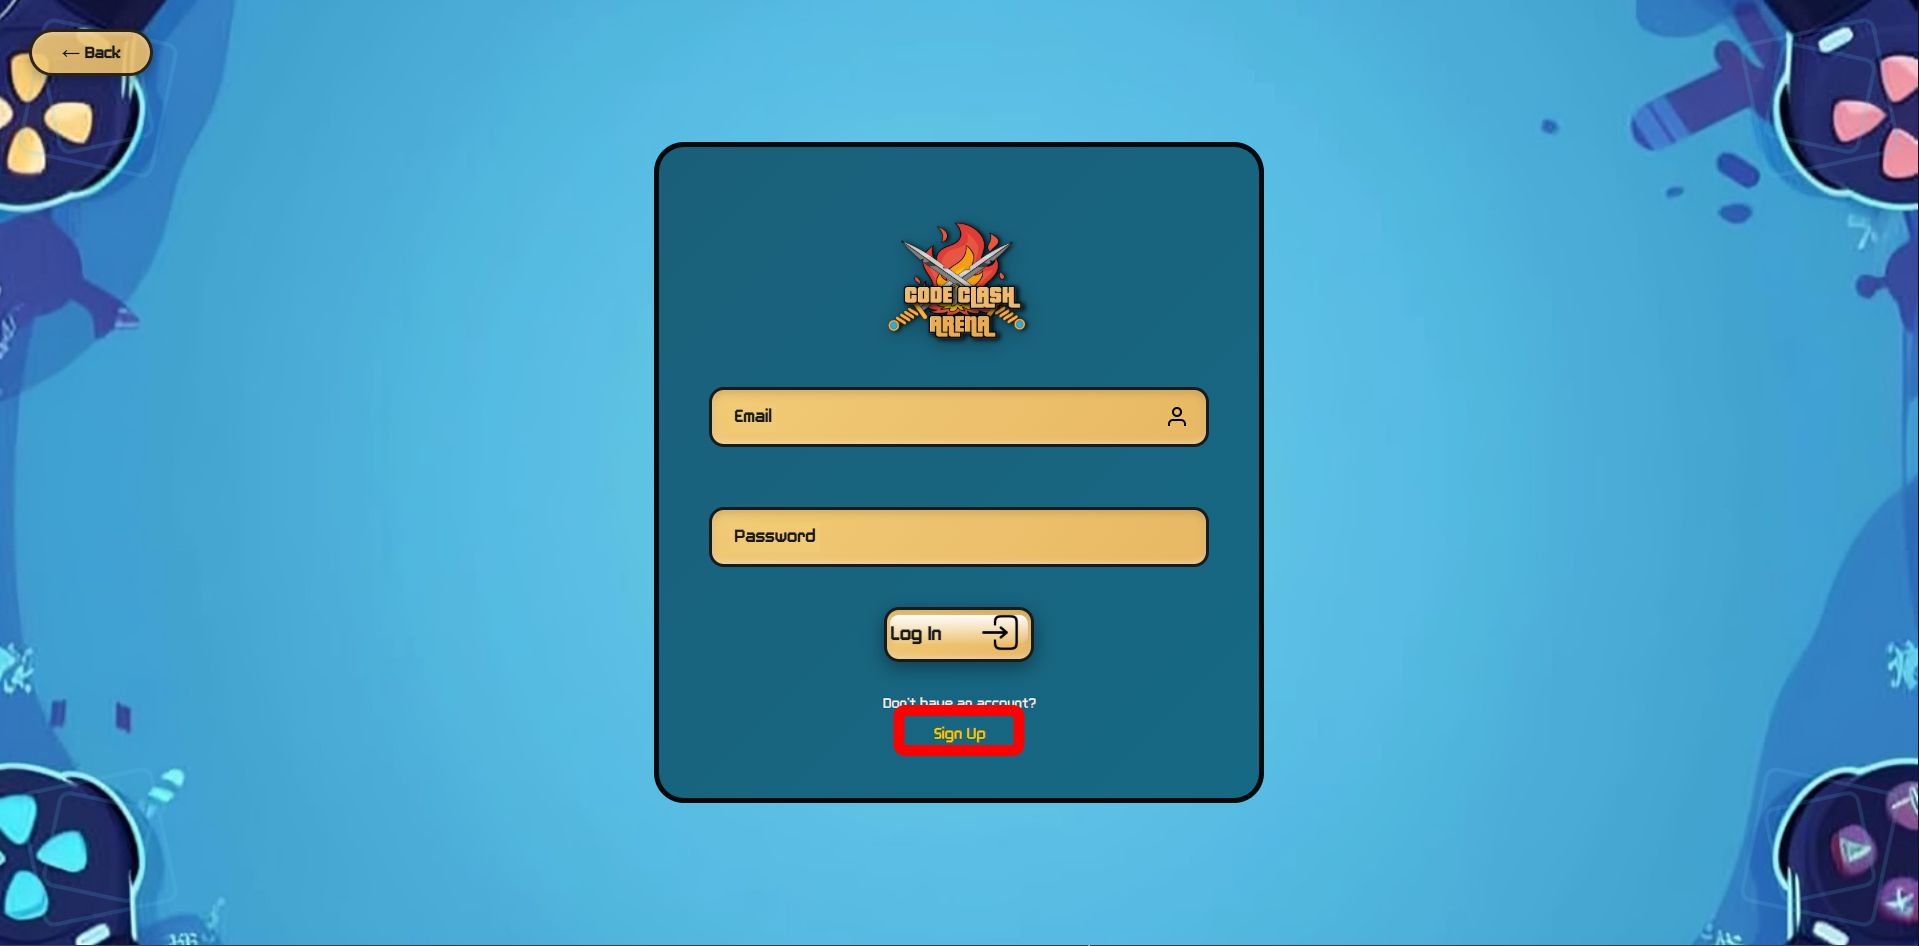
\includegraphics[width=0.95\textwidth]{homepage.png}
\caption{CodeClash Arena Loginpage - Locate Sign Up button}
\label{fig:homepage}
\end{figure}

\textbf{Step 2: Enter Registration Information}

Fill in all three required fields in the sign-up form:

\begin{itemize}[leftmargin=*]
\item \textbf{Email}: Provide a valid email address
  \begin{itemize}
    \item Used for account verification and password recovery
    \item Must be unique (not already registered in the system)
    \item Ensure you have access to this email for verification
    \item Format: username@domain.com
  \end{itemize}
\item \textbf{Codeforces Handle}: Enter your existing Codeforces username
  \begin{itemize}
    \item \textbf{This is your Codeforces account username} - not a new username
    \item Must be a valid, existing Codeforces handle
    \item This handle is linked immediately during registration
    \item Used for all code submissions and battle participation
    \item If you don't have a Codeforces account, create one first at \url{https://codeforces.com/register}
  \end{itemize}
\item \textbf{Password}: Create a strong password for your CodeClash Arena account
  \begin{itemize}
    \item Minimum 8 characters required
    \item Recommended: Include uppercase, lowercase, numbers, and special characters
    \item Password is case-sensitive
    \item This is separate from your Codeforces password
  \end{itemize}
\end{itemize}

\textbf{Important Note:} Unlike typical registrations, CodeClash Arena requires your Codeforces handle during sign-up because the platform integrates directly with Codeforces for problem sourcing and code submission.

\begin{figure}[!htb]
\centering
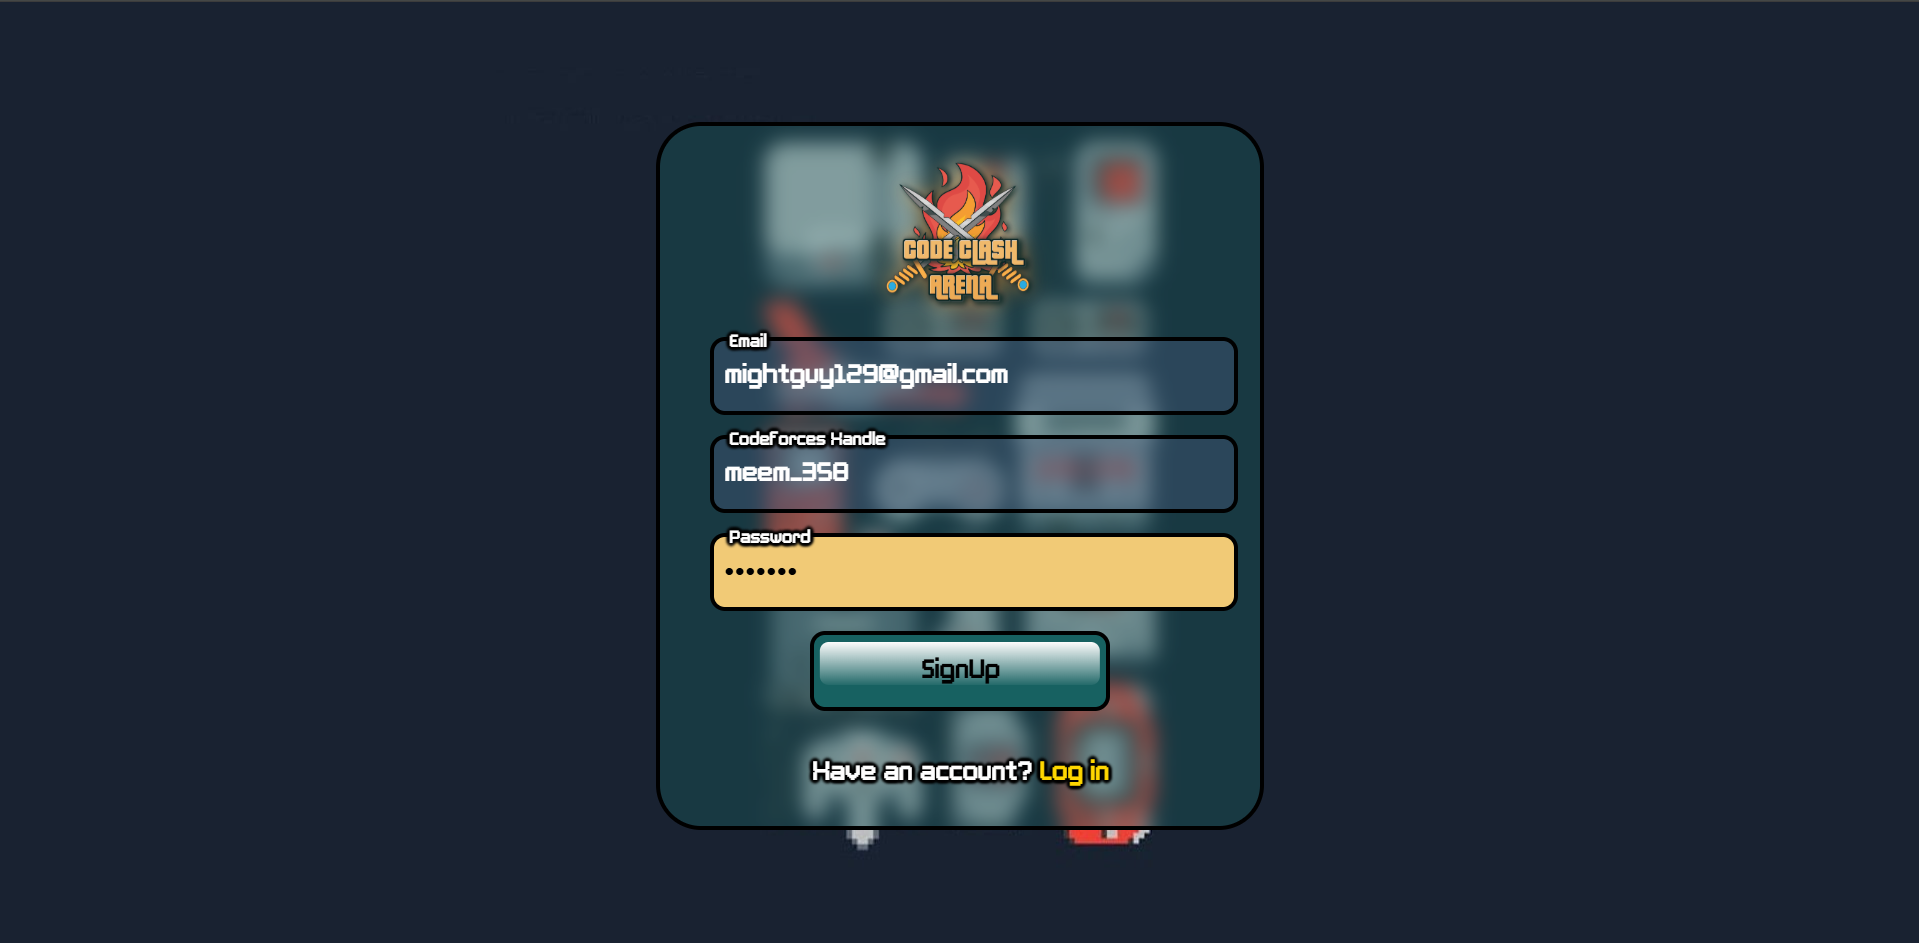
\includegraphics[width=0.9\textwidth]{signup_form.png}
\caption{Sign-Up Form - Enter registration details}
\label{fig:signup_form}
\end{figure}

\textbf{Step 3: Submit Registration}

\begin{itemize}[leftmargin=*]
\item Click the \textbf{"SignUp"} button (green/teal colored button)
\item The system will validate all entered information
\item If validation fails, field labels will turn red indicating errors:
  \begin{itemize}
    \item Red label on Email - Check email format or email may already be registered
    \item Red label on Codeforces Handle - Verify handle exists on Codeforces
    \item Red label on Password - Ensure password meets minimum requirements (8+ characters)
    \item Empty fields are highlighted in red when attempting to submit
  \end{itemize}
\item Upon successful validation, account creation begins
\end{itemize}

\begin{figure}[!htb]
\centering
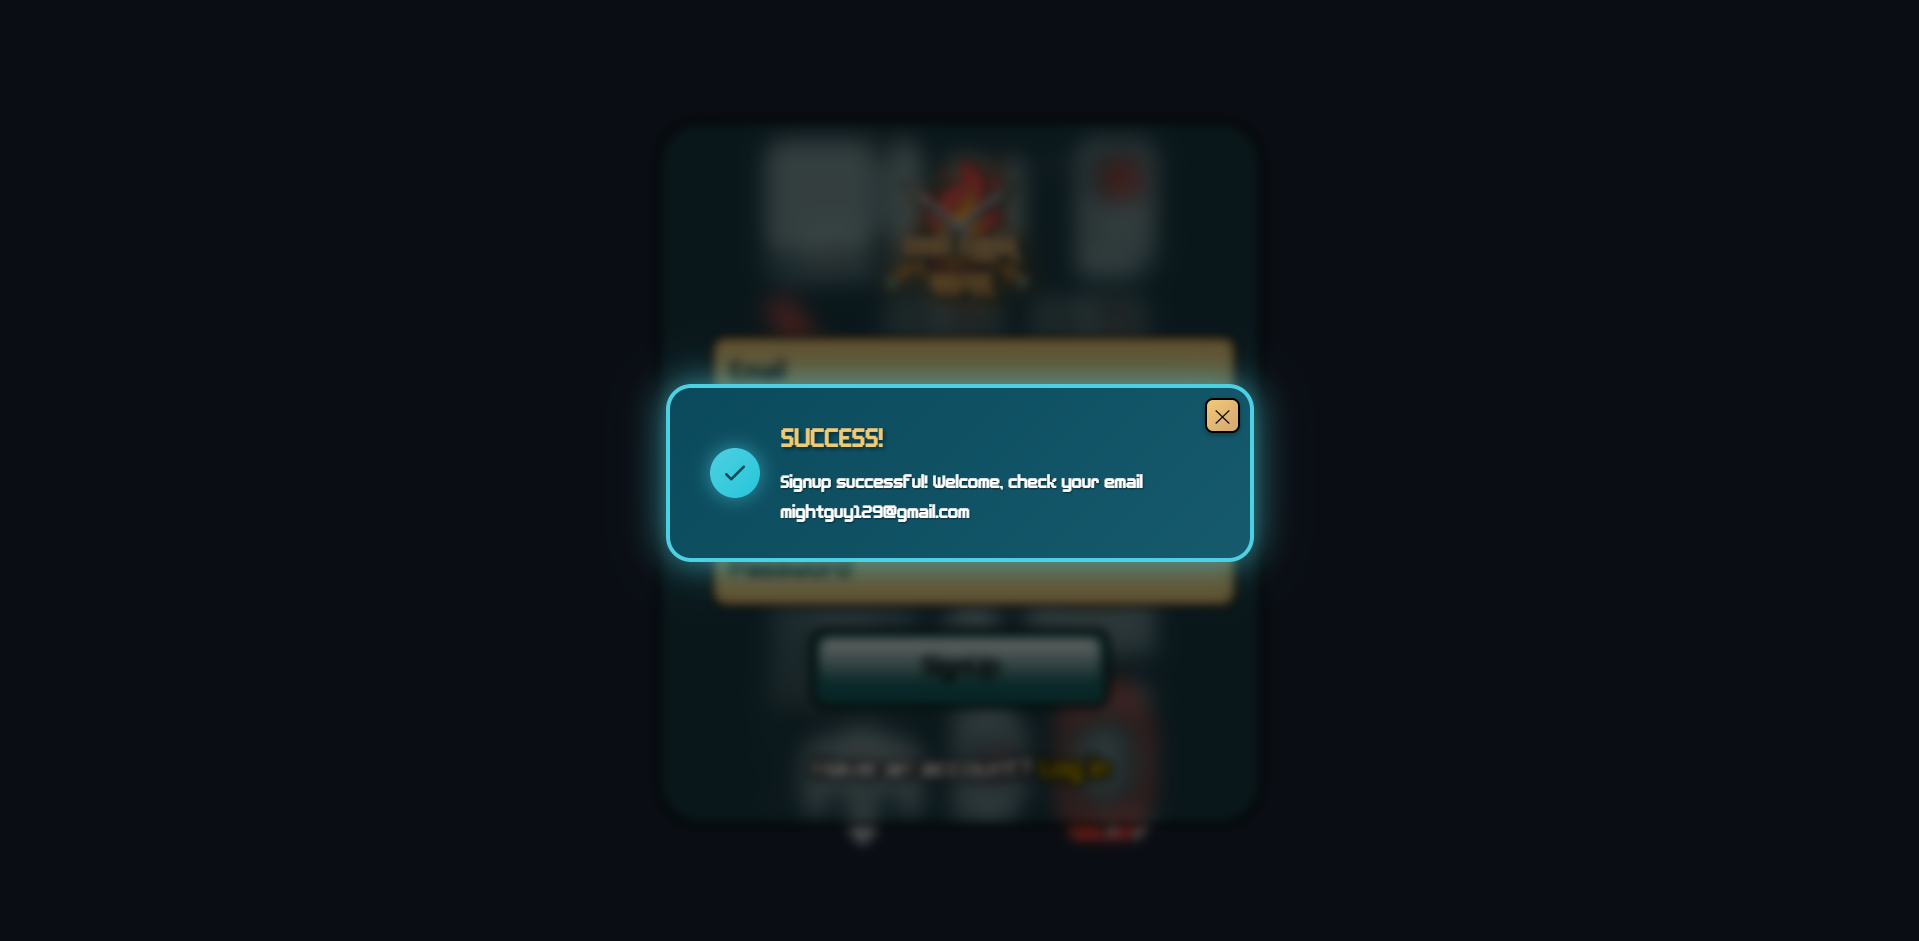
\includegraphics[width=0.9\textwidth]{signup_submit.png}
\caption{Sign-Up Form Completion - Click SignUp button}
\label{fig:signup_submit}
\end{figure}

\textbf{Step 4: Email Verification Alert}

\begin{itemize}[leftmargin=*]
\item After successful registration, a success alert popup appears with the message: \textbf{"Signup successful! Welcome, check your email [your-email@domain.com]"}
\item The page automatically redirects to the Homepage after 1.5 seconds
\item Check your email inbox for a verification message from Supabase (CodeClash Arena's authentication provider)
\item Subject line typically: "Confirm Your Email" or "Verify Your Email"
\item Email may take 1-5 minutes to arrive
\item Check spam/junk folder if email is not received within 5 minutes
\end{itemize}

\begin{figure}[!htb]
\centering
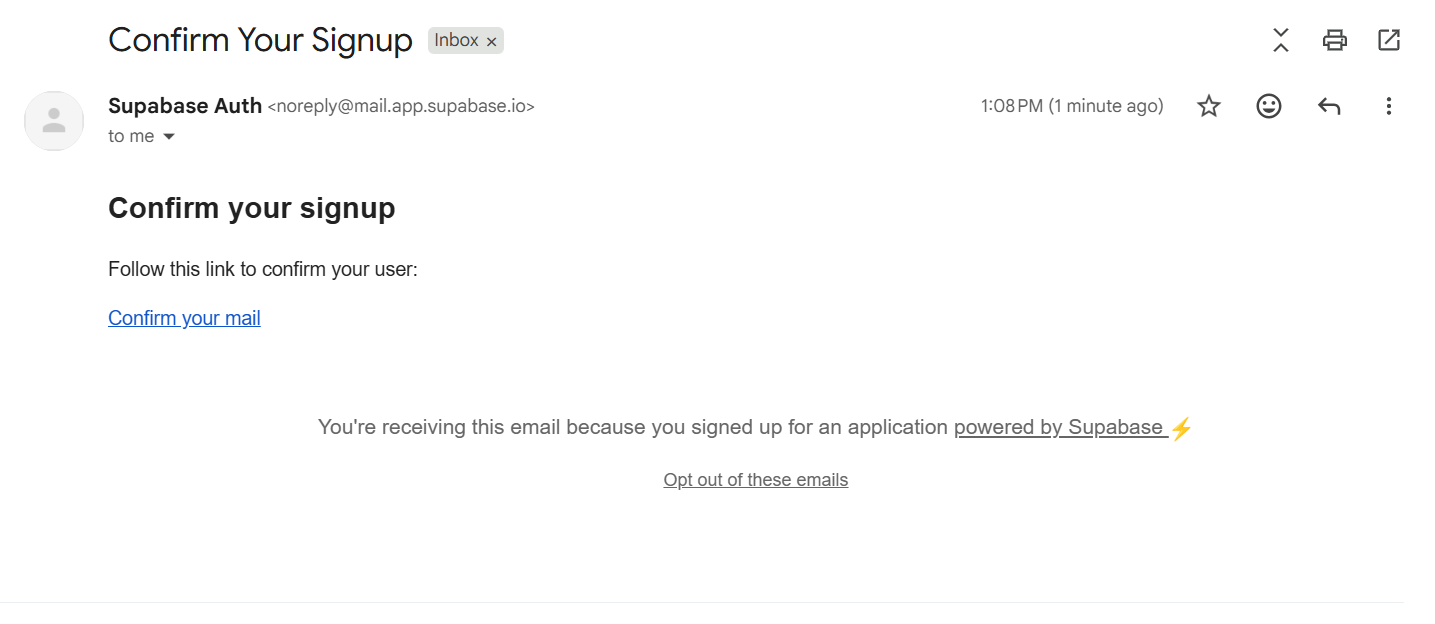
\includegraphics[width=0.9\textwidth]{verification_email.png}
\caption{Email Verification }
\label{fig:verification_prompt}
\end{figure}

\textbf{Step 5: Verify Email Address}

\begin{itemize}[leftmargin=*]
\item Open the verification email
\item Click on the \textbf{"Verify Email Address"} button or link
\item Browser will open and redirect to CodeClash Arena
\item Verification confirmation page appears
\item Account is now fully activated
\end{itemize}

\textbf{Step 6: Login to Complete Setup}

After email verification:
\begin{itemize}[leftmargin=*]
\item Navigate to the Login page
\item Login using your registered email and password
\item Your Codeforces handle is already linked from registration
\item You can now access all platform features including battles, practice gym, and clan wars
\end{itemize}

\textbf{Important Notes:}
\begin{itemize}[leftmargin=*]
\item \textbf{Codeforces Handle Required First}: You must have an existing Codeforces account before signing up on CodeClash Arena
\item \textbf{Verification Link Expiry}: Email verification links typically expire after 24 hours
\item \textbf{Unverified Accounts}: You must verify your email to login and access platform features
\item \textbf{Handle Validation}: The system stores your Codeforces handle but doesn't validate its existence during registration - ensure you enter it correctly
\item \textbf{Account Security}: Never share your CodeClash Arena password with anyone (keep it separate from your Codeforces password)
\item \textbf{Success Alert}: Green alert popup confirms successful registration
\item \textbf{Error Alert}: Red alert popup displays error messages if registration fails
\end{itemize}

\FloatBarrier

\subsection{Login Process}

Existing users can access their accounts through the login page. The process is quick and secure.

\subsubsection{Login Steps}

\textbf{Step 1: Navigate to Login Page}

\begin{itemize}[leftmargin=*]
\item From the homepage, click the \textbf{"GET STARTED"} button
\item You will be automatically redirected to the Login page
\item Alternatively, navigate directly via your browser if you know the URL
\item The login page displays with the CodeClash Arena logo at the top
\item A \textbf{"← Back"} button is available in the top-left corner to return to the homepage
\end{itemize}

\begin{figure}[!htb]
\centering
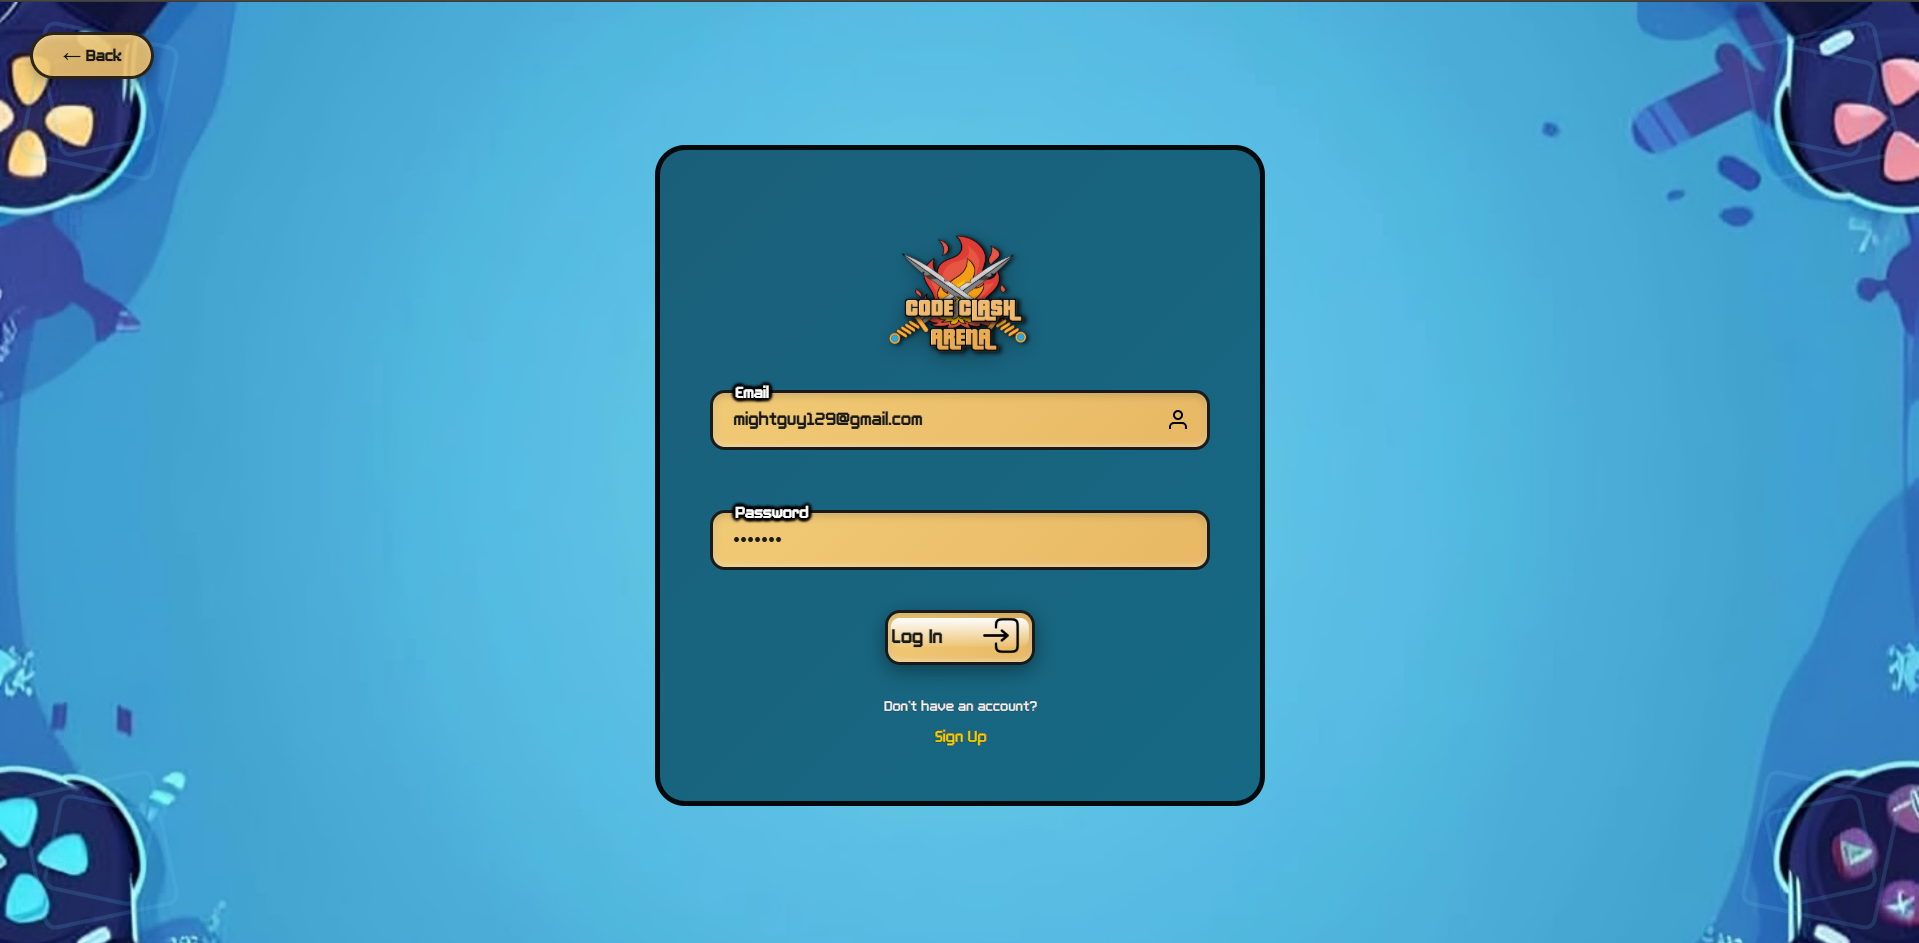
\includegraphics[width=0.95\textwidth]{loginpage.png}
\caption{Loginpage - Navigate to Login}
\label{fig:homepage_login}
\end{figure}

\textbf{Step 2: Enter Login Credentials}

\begin{itemize}[leftmargin=*]
\item \textbf{Email Field}: Enter the email address used during registration
  \begin{itemize}
    \item Labeled as "Email" with a user icon on the left
    \item Email is case-insensitive
    \item Ensure no extra spaces before or after email
    \item Floating label design - label moves up when you start typing
  \end{itemize}
\item \textbf{Password Field}: Enter your account password
  \begin{itemize}
    \item Labeled as "Password" with floating label design
    \item Password is case-sensitive
    \item Click on the password field to focus it
    \item When focused, an \textbf{eye icon} appears on the right side
    \item Click the eye icon to toggle password visibility (show/hide)
    \item Closed eye icon = password hidden; Open eye icon = password visible
  \end{itemize}
\end{itemize}

\textbf{Step 3: Submit Login}

\begin{itemize}[leftmargin=*]
\item Click the \textbf{"Log In"} button (golden/yellow colored button with login icon)
\item System validates credentials with Supabase authentication service
\item Authentication typically completes within 1-2 seconds
\item Success or error alert popup will appear
\end{itemize}

\begin{figure}[!htb]
\centering
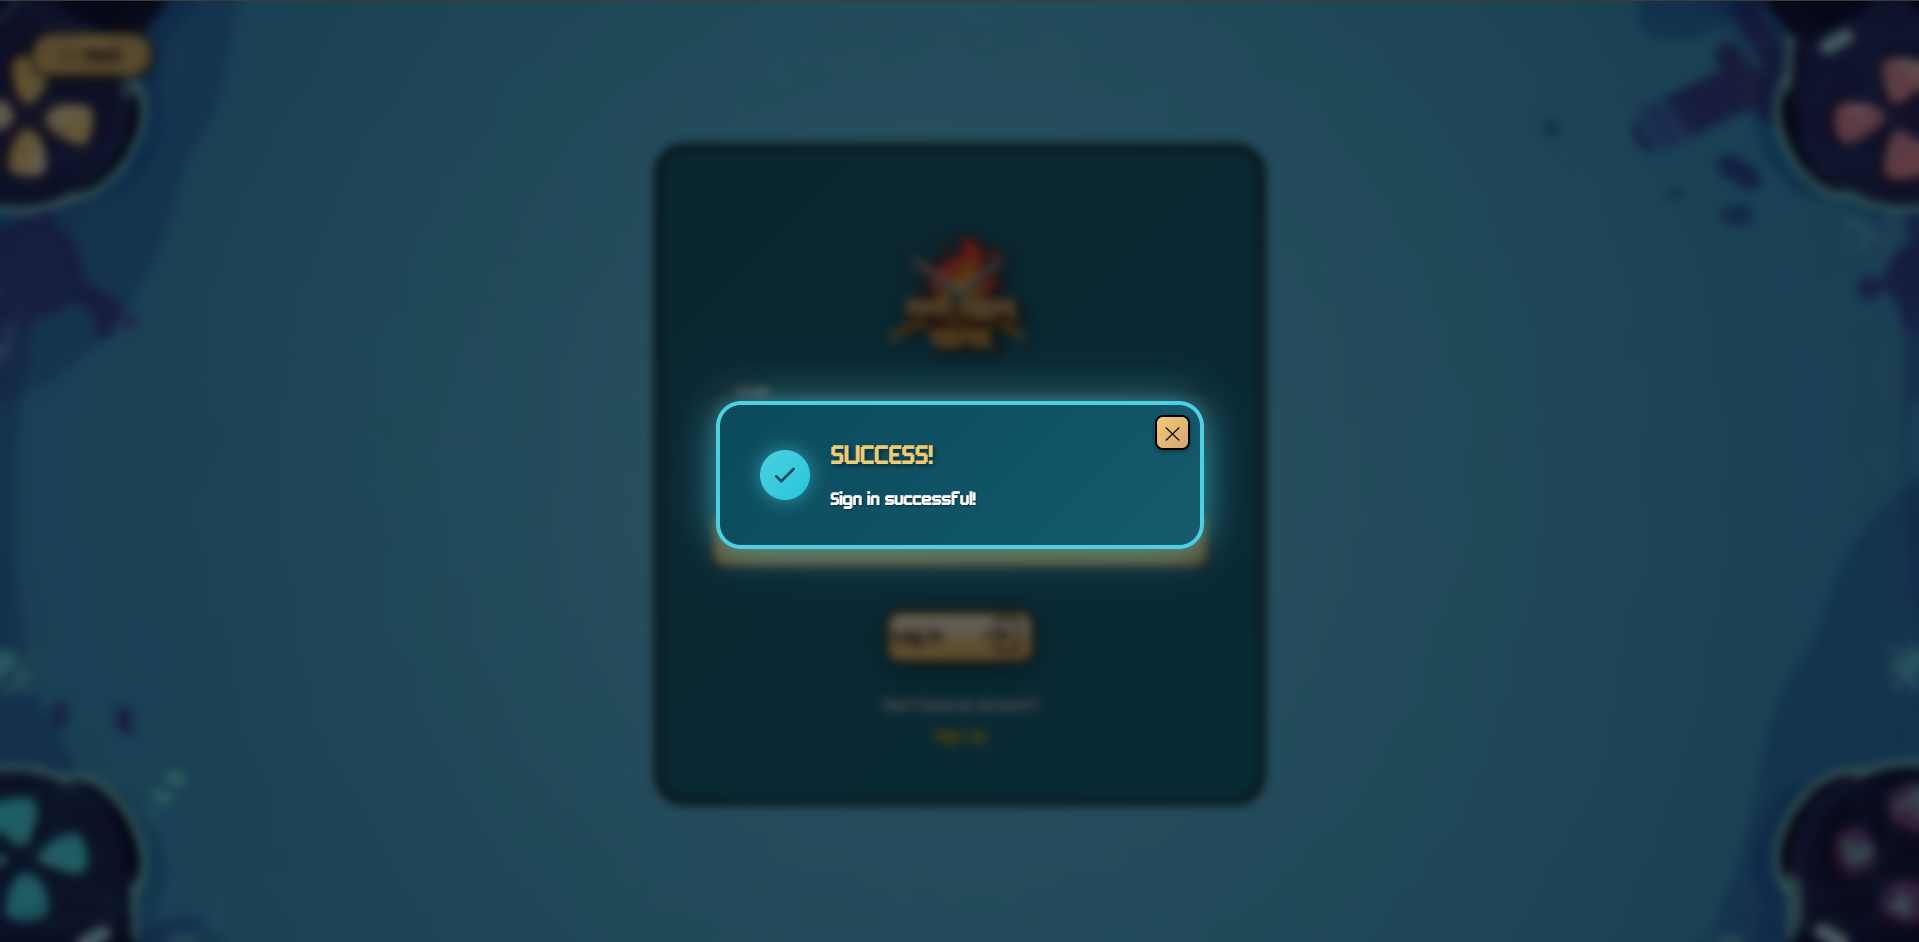
\includegraphics[width=0.9\textwidth]{login_submit.png}
\caption{Login successful - Success alert displayed}
\label{fig:login_success}
\end{figure}

\textbf{Step 4: Successful Login - Redirection}

\begin{itemize}[leftmargin=*]
\item Upon successful authentication, a green success alert appears: \textbf{"Sign in successful!"}
\item After 1.5 seconds, you are automatically redirected to the \textbf{Main Dashboard} (/main)
\item Your Codeforces handle is automatically loaded from the database and stored in browser localStorage
\item Navigation bar updates to show logged-in status with your profile information
\item Access to all platform features is now available: PvP Battles, Practice Gym, Clan Wars, Leaderboards
\end{itemize}

\begin{figure}[!htb]
\centering
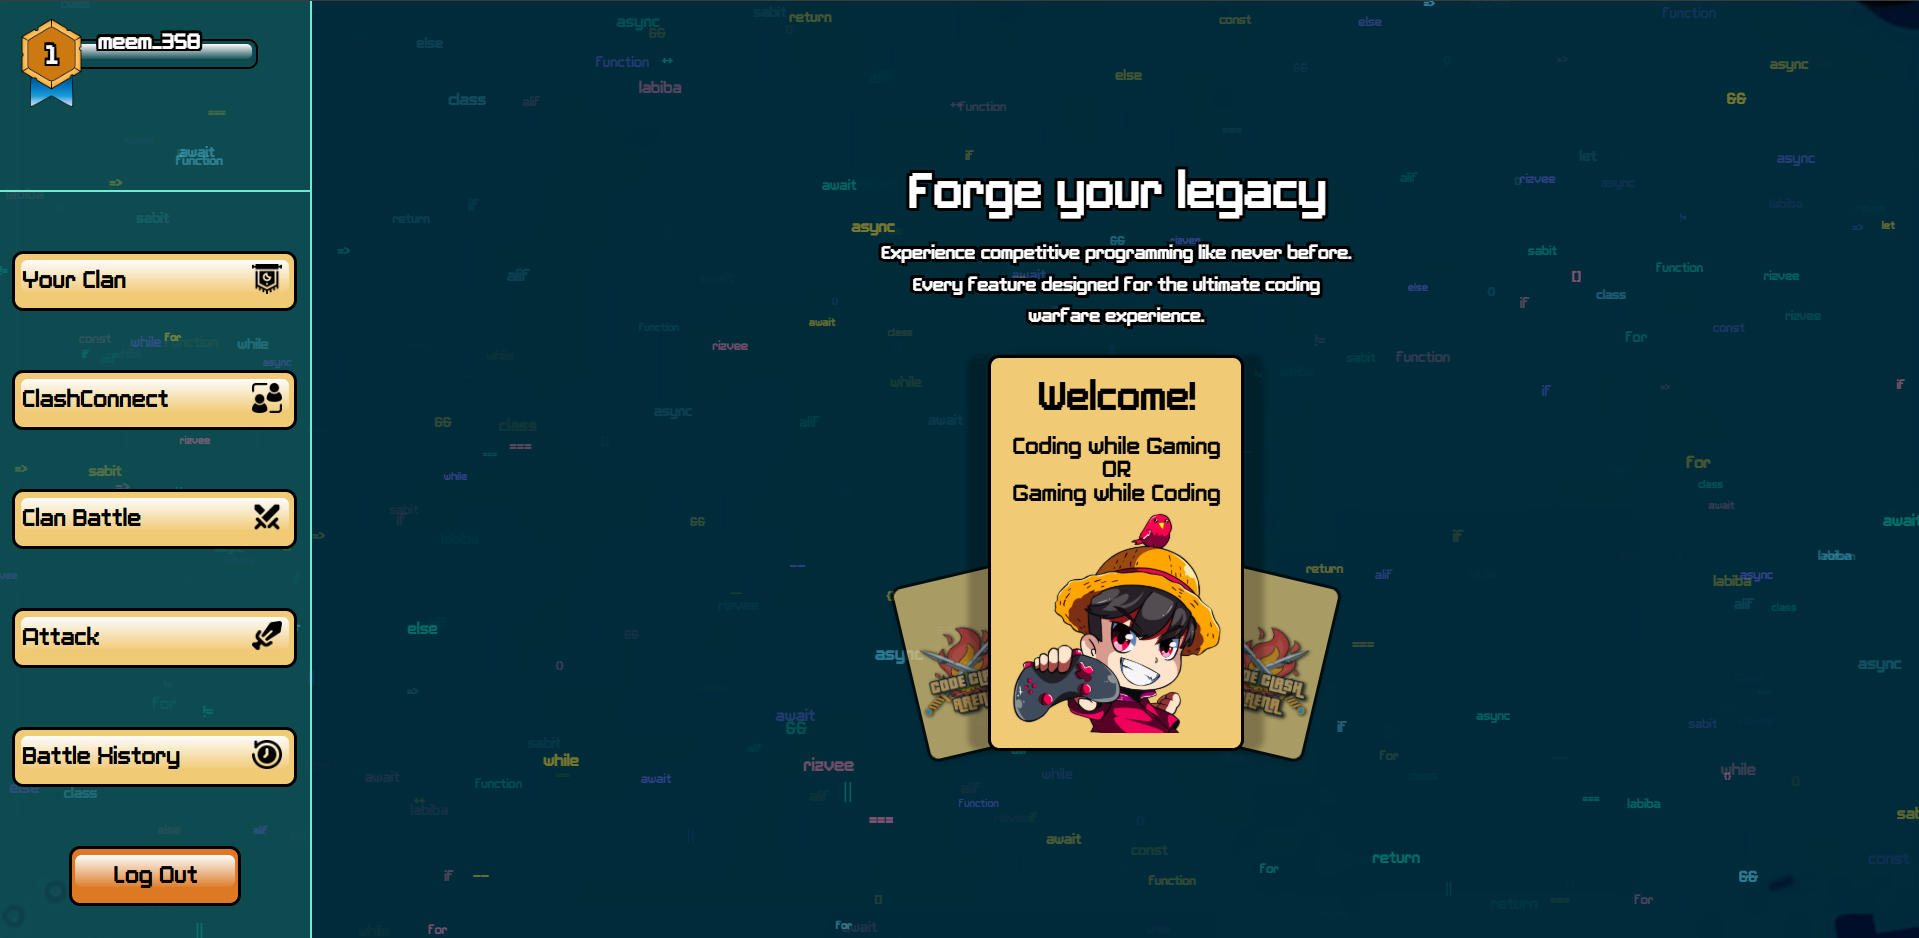
\includegraphics[width=0.95\textwidth]{maindasboard.png}
\caption{Main Dashboard - After successful login}
\label{fig:dashboard}
\end{figure}

\textbf{Common Login Errors and Solutions:}

\begin{longtable}{|p{5cm}|p{8.5cm}|}
\hline
\textbf{Error Message} & \textbf{Solution} \\
\hline
\endhead

"Invalid email or password" or authentication error & Verify email and password are correct; check for typos; ensure Caps Lock is off; verify email has been verified via link sent during signup \\
\hline

"Email not verified" & Check your email inbox for verification link; you must verify email before logging in; check spam/junk folder \\
\hline

"Account not found" & Email may not be registered; try signing up or verify correct email address \\
\hline

"Too many login attempts" & Wait 15 minutes before trying again; security measure against brute force attacks \\
\hline

"Network error" & Check internet connection; ensure stable connectivity; try refreshing page \\
\hline

\end{longtable}

\subsubsection{First-Time Login - Account Setup Complete}

After your first successful login:

\textbf{Codeforces Account Already Linked:}
\begin{itemize}[leftmargin=*]
\item Your Codeforces handle was linked during the sign-up process
\item No additional Codeforces setup is required
\item The system automatically retrieves your cf\_handle from the database upon login
\item This handle is used for all code submissions to Codeforces during battles
\item You can proceed immediately to explore the platform features
\end{itemize}

\textbf{If You Need to Update Codeforces Handle:}
\begin{enumerate}
\item Navigate to \textbf{Profile Settings} or \textbf{User Profile} section
\item Locate the \textbf{"Codeforces Handle"} field
\item Update your Codeforces username/handle if needed
\item Save changes
\item Note: Handle changes may be rate-limited to prevent abuse
\end{enumerate}


\textbf{Important}: Without a linked Codeforces account, you cannot participate in competitive battles or submit code solutions.

\FloatBarrier

\subsection{Logout Process}

Users can securely log out of their accounts at any time to end their session.

\subsubsection{Logout Steps}

\textbf{Step 1: Access User Menu}

\begin{itemize}[leftmargin=*]
\item Locate your username or profile icon in the top-right corner of the navigation bar
\item Click on the username/profile icon to open the dropdown menu
\item User menu will display with various options
\end{itemize}

\begin{figure}[!htb]
\centering
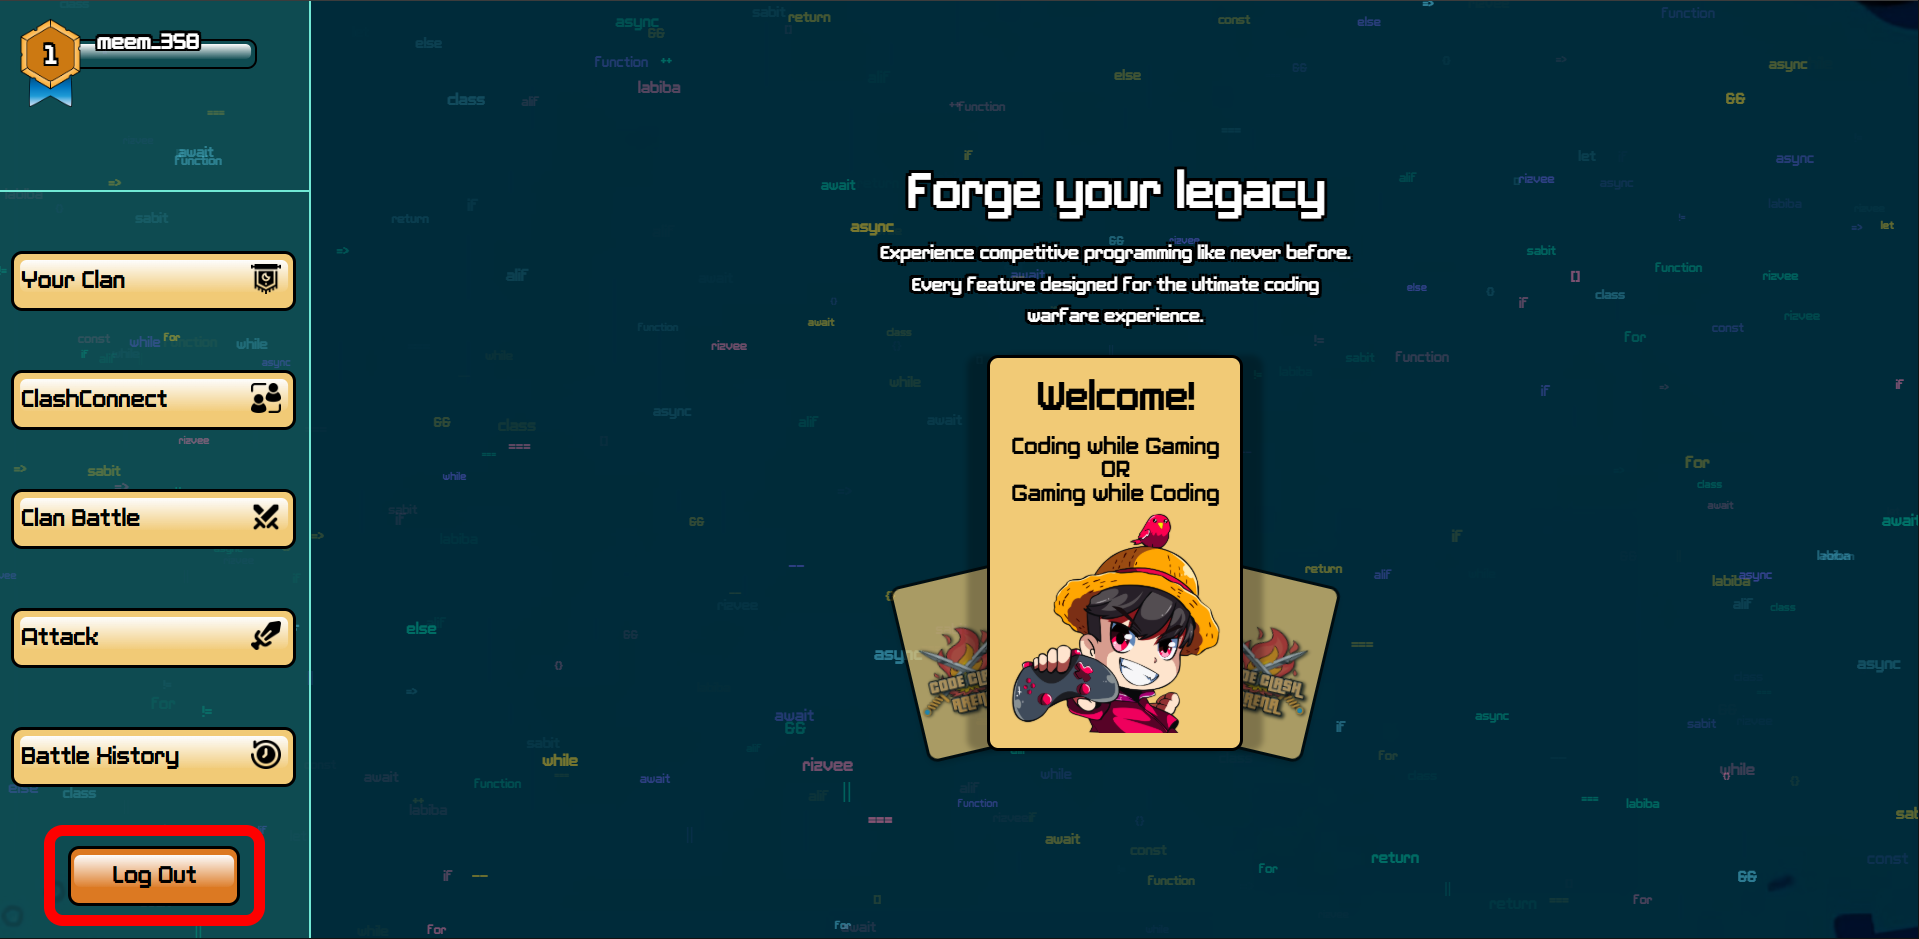
\includegraphics[width=0.9\textwidth]{logout.png}
\caption{User Menu - Access logout option}
\label{fig:user_menu}
\end{figure}

\textbf{Step 2: Select Logout Option}

\begin{itemize}[leftmargin=*]
\item From the dropdown menu, locate and click \textbf{"Logout"} or \textbf{"Sign Out"}
\item Option is typically at the bottom of the menu
\item May be represented by a logout icon (exit door or arrow)
\end{itemize}

\textbf{Step 3: Confirm Logout (if applicable)}

\begin{itemize}[leftmargin=*]
\item Confirmation dialog may appear: "Are you sure you want to logout?"
\item Click \textbf{"Yes"} or \textbf{"Confirm"} to proceed
\item Click \textbf{"Cancel"} to remain logged in
\item Some implementations may log out immediately without confirmation
\end{itemize}

\textbf{Step 4: Logout Completion}

\begin{itemize}[leftmargin=*]
\item Session is terminated on the server
\item Authentication tokens are cleared from browser
\item You are redirected to the homepage or login page
\item Confirmation message appears: "Successfully logged out"
\item All session data is cleared for security
\end{itemize}



\textbf{Important Security Notes:}
\begin{itemize}[leftmargin=*]
\item \textbf{Always logout on shared computers}: Prevent unauthorized access to your account
\item \textbf{Battle interruption}: If logged out during an active battle, it counts as forfeit
\item \textbf{Unsaved changes}: Any unsaved draft code in editor may be lost
\item \textbf{Session persistence}: "Remember Me" option keeps you logged in until explicit logout
\item \textbf{Automatic logout}: Sessions may expire after extended inactivity (typically 24-48 hours)
\end{itemize}

\FloatBarrier

\subsection{Troubleshooting Common Issues}

\subsubsection{Cannot Receive Verification/Reset Emails}

\textbf{Solutions:}
\begin{itemize}[leftmargin=*]
\item Check spam/junk folder for emails from Supabase
\item Verify email address was entered correctly during signup
\item Wait 5-10 minutes (email delivery may be delayed)
\item Whitelist emails from your authentication provider
\item Check email provider's filtering settings
\item Contact platform support if verification email is never received
\end{itemize}

\subsubsection{Account Locked After Multiple Failed Login Attempts}

\textbf{Solutions:}
\begin{itemize}[leftmargin=*]
\item Wait 15-30 minutes before attempting to login again
\item Ensure correct email and password are being used
\item Use password reset if password is forgotten
\item Contact support if issue persists after waiting period
\end{itemize}

\subsubsection{Browser Compatibility Issues}

\textbf{Solutions:}
\begin{itemize}[leftmargin=*]
\item Update browser to minimum required version (Chrome 84+, Firefox 103+, Safari 15+)
\item Enable JavaScript in browser settings
\item Clear browser cache and cookies
\item Disable browser extensions that may interfere
\item Try using a different supported browser
\end{itemize}

\subsection{Next Steps After Getting Started}

Once successfully logged in, proceed to:

\begin{enumerate}
\item \textbf{Explore Main Dashboard}: Familiarize yourself with navigation menu and available features - PvP Battles, Practice Gym, Clan Wars, and more
\item \textbf{Verify Codeforces Handle}: Your Codeforces handle was linked during signup - verify it appears correctly in your profile
\item \textbf{Complete Profile}: Add additional information, avatar, or bio (if available in profile settings)
\item \textbf{Browse Practice Gym}: Start with practice problems to familiarize yourself with the code editor and problem-solving interface
\item \textbf{Join or Create a Clan}: Team up with other coders for clan battles and collaborative competitions (optional)
\item \textbf{Enter First Battle}: Once comfortable, try a 1v1 PvP battle to experience competitive real-time coding
\end{enumerate}

\textbf{Recommended First Actions:}
\begin{itemize}[leftmargin=*]
\item Visit the \textbf{Practice Gym} to try solving a problem without time pressure
\item Check the \textbf{Leaderboard} to see top-ranked players
\item Read platform tutorials or help section (if available)
\item Configure notification preferences in settings
\end{itemize}

\FloatBarrier

% ==================================================
% SECTION 4: USER ROLES
% ==================================================

\section{User Roles}

CodeClash Arena is designed exclusively for authenticated registered users to ensure fair participation in competitive coding battles. Access to the platform requires account creation, email verification, and a linked Codeforces handle. There are no guest or admin roles in the system - all users have equal access to platform features and compete on a level playing field based on their coding skills and performance.

\subsection{Registered User}

A registered user is any individual who has successfully completed the sign-up process, verified their email address, and linked a valid Codeforces handle to their account. This is the only role on the platform, and all authenticated users operate with the same base permissions.

\subsubsection{Permissions}

Registered users have access to the following platform features:

\begin{itemize}[leftmargin=*]
\item \textbf{Account Management}: Register an account with email and Codeforces handle, log in and log out securely, update profile information and preferences
\item \textbf{Real-Time 1v1 Coding Battles}: Participate in Local battles (challenge specific friends with custom settings), participate in Global battles (matchmaking with players of similar skill level), compete in time-based coding challenges with live synchronization
\item \textbf{Clan System}: Create a new clan or join existing clans, participate in clan battles when selected by clan leader, contribute to clan rankings and statistics, manage clan memberships (leaders can approve/reject join requests)
\item \textbf{Code Submission}: Submit code solutions in multiple programming languages (C++, Java, Python, JavaScript, etc.), receive automated verdicts from Codeforces judge (Accepted, Wrong Answer, Time Limit Exceeded, etc.), test code locally using integrated code editor
\item \textbf{Statistics and Rankings}: View personal battle history and performance metrics, track XP, level, and ELO-based rating progression, access global and clan leaderboards, view detailed submission verdicts and problem-solving statistics
\item \textbf{Practice Mode}: Access Practice Gym with thousands of Codeforces problems, filter problems by difficulty, tags, and rating range, receive AI-based logical hints for approach guidance (without revealing full solutions), solve problems without time pressure for skill improvement
\item \textbf{Social Features}: Send and accept friend requests, view friend profiles and statistics, receive notifications for clan join requests and battle invitations
\end{itemize}

\subsubsection{Restrictions}

Registered users are subject to the following restrictions to maintain platform integrity and fair competition:

\begin{itemize}[leftmargin=*]
\item \textbf{No System Modifications}: Users cannot modify system configurations, settings, or platform code
\item \textbf{No Ranking Manipulation}: Direct manipulation of ratings, XP, leaderboards, or battle outcomes is strictly prohibited
\item \textbf{No Private Data Access}: Users cannot access other users' private information, submission code, or system database records
\item \textbf{No Unauthorized Authentication}: Users cannot share accounts or use multiple accounts to gain unfair advantages
\item \textbf{Fair Play Requirements}: Code submissions must be original work; plagiarism or copying solutions is not permitted
\end{itemize}

\FloatBarrier

% ==================================================
% SECTION 5: FEATURES AND FUNCTIONALITY
% ==================================================

\section{Features and Functionality}
% To be completed in next iteration

\FloatBarrier

% ==================================================
% SECTION 6: NAVIGATION GUIDE
% ==================================================

\section{Navigation Guide}

This section provides a comprehensive guide to navigating CodeClash Arena's interface. After logging in, you will be directed to the Main Dashboard, which serves as the central hub for accessing all platform features.

\subsection{Main Dashboard Overview}

The Main Dashboard features an animated background with coding-themed particles and a vertical menu bar on the left side. At the top of the menu, you will see your XP bar displaying your current level, experience points, and username. Below the XP bar are five main navigation buttons and a logout option.

\subsection{Navigation Options}

\subsubsection{Your Clan}

Access your clan management interface and view clan details. If you are not currently in a clan, clicking this button opens the clan browsing menu where you can search for clans to join or create your own clan. If you are already a clan member, this opens your clan's information page showing member list, clan statistics, total points, and war history.

\subsubsection{ClashConnect}

Open the social hub to manage your connections and invitations. This feature allows you to search for other players, send and accept friend requests, view incoming clan join requests (if you are a clan leader), and manage your friend list. A notification badge appears on this button when you have pending friend requests or clan join requests.

\subsubsection{Clan Battle}

Navigate to the clan battle interface for team-based competitions. If you are a clan leader, clicking this button takes you to the team selection page where you can choose warriors and initiate matchmaking for clan battles. If you are a regular clan member and a battle is ongoing, you will be directed to the battle arena; otherwise, you will see a "No Battle Ongoing" message. A notification badge appears when there is an active clan battle.

\subsubsection{Attack}

Launch the PvP battle menu to compete in 1v1 coding challenges. This button opens an overlay menu with multiple battle mode options: Global Battle Mode (matchmaking with players of similar rating), Local Battle Mode (challenge specific friends), and Practice Gym (solo practice without competition). Select your preferred mode to begin competitive coding.

\subsubsection{Battle History}

View your complete battle record and performance statistics. This section displays all your past 1v1 battles and clan battles, showing opponents faced, problems solved, battle outcomes (win/loss), time taken, and rating changes. Use this feature to analyze your performance trends and track your improvement over time.

\subsubsection{Log Out}

Securely end your current session and return to the homepage. Clicking this button clears your authentication tokens and logs you out of the platform. Always use this option when accessing CodeClash Arena from shared or public computers to protect your account security.

\FloatBarrier

% ==================================================
% SECTION 7: ERROR HANDLING AND MESSAGES
% ==================================================

\section{Error Handling and Messages}

CodeClash Arena displays color-coded alerts to communicate system status: green alerts for successful actions (e.g., "Sign in successful!") and red alerts for errors. Alerts disappear automatically after a few seconds or can be manually closed.

\subsection{Authentication Errors}

\textbf{Invalid Login Credentials}

\textit{Error Message:} "Invalid login credentials" or "Invalid email or password"

\textit{Solutions:} Verify email and password are correct; check Caps Lock is off; ensure no extra spaces; use correct email (not Codeforces handle); verify email has been confirmed after signup.

\textbf{Email Not Confirmed/Verified}

\textit{Error Message:} "Email not confirmed" or "Error fetching user data"

\textit{Solutions:} Check inbox and spam folder for verification email from Supabase; look for subject "Confirm Your Email"; click verification link; return to login page after verification; contact support if link expired (24 hours).

\textbf{Account Locked}

\textit{Error Message:} "Too many login attempts"

\textit{Solutions:} Wait 15-30 minutes before retrying; use password reset if needed; avoid multiple attempts during lockout.

\textbf{Email Already Registered}

\textit{Error Message:} "User already registered" or "Email already exists"

\textit{Solutions:} Use login page if account exists; use password reset if password forgotten; try different email for new account.

\textbf{Invalid Codeforces Handle}

\textit{Error Message:} Field validation error or "Invalid handle"

\textit{Solutions:} Verify handle at \url{https://codeforces.com/profile/your-handle}; ensure exact spelling and capitalization; create Codeforces account first if needed.

\textbf{Weak Password}

\textit{Error Message:} "Password must be at least 8 characters"

\textit{Solutions:} Use minimum 8 characters with mix of uppercase, lowercase, numbers, and special characters; avoid common passwords.

\subsection{Network and Connectivity Errors}

\textbf{Network Error:} "Network error" or "Failed to fetch"

\textit{Solutions:} Check internet connection; refresh page (F5); verify firewall settings; disable VPN temporarily; clear browser cache; try different browser.

\textbf{Timeout Error:} "Request timeout" or "Connection timeout"

\textit{Solutions:} Ensure stable connection (5+ Mbps for battles); close bandwidth-consuming applications; switch to wired connection; try again after a moment.

\subsection{Battle-Related Errors}

\textbf{Battle Disconnection:} "Connection lost" or "Battle disconnected"

\textit{Note:} Automatic forfeit if reconnection fails.

\textit{Prevention:} Use wired Ethernet connection; ensure stable internet before battles; close unnecessary applications; avoid battles during network instability.

\textbf{Submission Failed:} "Submission failed" or "Error submitting code"

\textit{Solutions:} Check internet connection; verify Codeforces handle is correctly linked; ensure Codeforces account is in good standing; retry after a few seconds; verify correct programming language selected.

\subsection{Clan-Related Errors}

\textbf{Cannot Join Clan:} "Already in a clan" or "Join request failed"

\textit{Solutions:} Leave current clan before joining another; wait for pending requests to be processed; verify clan is accepting members and you meet requirements.

\textbf{Cannot Start Clan Battle:} "Insufficient permissions" or "Only clan leader can start battles"

\textit{Solutions:} Contact clan leader to start battle; create your own clan for leadership permissions.

\subsection{Common Error Messages Quick Reference}

\begin{longtable}{|p{6cm}|p{8cm}|}
\hline
\textbf{Error Message} & \textbf{Quick Solution} \\
\hline
\endhead

"Invalid login credentials" & Check email and password; ensure credentials correct; verify email confirmed \\
\hline

"Email not confirmed" / "Error fetching user data" & Check inbox for verification email; click verification link; check spam folder \\
\hline

"Network error" & Check internet; refresh page; verify firewall settings \\
\hline

"User already registered" & Use login instead; try different email; reset password if needed \\
\hline

"Too many login attempts" & Wait 15-30 minutes before retry \\
\hline

"Submission failed" & Check internet; verify Codeforces handle linked; retry submission \\
\hline

"Connection timeout" & Improve internet stability; use wired connection; close other apps \\
\hline

"Battle disconnected" & Ensure stable internet before battles; use wired connection \\
\hline

"Already in a clan" & Leave current clan first \\
\hline

"Only clan leader can start battles" & Contact clan leader or create own clan \\
\hline

"Password must be at least 8 characters" & Use longer password with mixed characters (uppercase, lowercase, numbers, symbols) \\
\hline

\end{longtable}



\FloatBarrier

% ==================================================
\end{document}
